%%%%%%%%%%%%%%%%%%%%%%%%%%%%%%%%%%%%%%%%%%%%%%%%%%%%%%%%%%%%%%%%%%%%%%%%%%%%%%%%%%%%%%
% TEMPLATE FOR Praktikum P3B
% This template uses the Memoir class. It is a very powerful class for creating documents such
% as reports, papers and theses. You can find more information at CTAN, the Comprehensive
% TeX Archive Network. These is a long manual that describes how to use Memoir.
% https://www.ctan.org/pkg/memoir?lang=en
% Sven Buschke
% Last Update: 2021-08-18
%%%%%%%%%%%%%%%%%%%%%%%%%%%%%%%%%%%%%%%%%%%%%%%%%%%%%%%%%%%%%%%%%%%%%%%%%%%%%%%%%%%%%

%------------------------------------------------------------------------------------
%	EDIT THIS BLOCK
%------------------------------------------------------------------------------------
\newcommand{\studentfullname}{Sven Buschke}			% change to your name
\newcommand{\matrikelnumber}{27205317}				% enter your student number 
\newcommand{\dateexperiment}{31. August 2021}				% change to your partner's name
\newcommand{\timeexperiment}{8:30-13:30 Uhr}				% enter your partner's student number
\title{P3B-Versuch 3C NMR-B --- Gepulste Kernspinresonanz}					% change to the title of the experiment
\author{\studenfullname}				% you don't have to change this
\date{30.\ August 2021}										% this fills in today's date - don't change



%------------------------------------------------------------------------------------
%	FORMATTING STUFF
%------------------------------------------------------------------------------------

\documentclass[12pt,oneside,oldfontcommands]{memoir}


%-----------------------------------------------------------------------------------
%	MARGIN AND HEADER/FOOTER SIZES
%------------------------------------------------------------------------------------
\setlrmarginsandblock{2.5cm}{2.5cm}{*}  		% left/right margins
\setulmarginsandblock{2.5cm}{2.5cm}{*} 			% top/bottom margins
\checkandfixthelayout							% checks the layout is correct
\setlength{\parindent}{0in}  					% no indent on start of paragraph
							

%-------------------------------------------------------------------------------------
%  PACKAGES
%-------------------------------------------------------------------------------------
\usepackage{amsmath,amsthm,amssymb,amsfonts}			% math fonts
\usepackage[german]{babel}								% hyphenation rules for German
\usepackage{graphicx}									% for importing pdf files 
\usepackage{siunitx}									% si units - extremely useful
\usepackage[usenames,dvipsnames,svgnames,table]{xcolor}	% defines the dvips color names
\usepackage{color,soul} 								% for highlight hi - hyphenation, underlining
%\usepackage{libertine}
%\usepackage{libertinust1math}
%\usepackage[T1]{fontenc}
\usepackage{fontspec}
\usepackage{pdfpages}
\setmainfont{Linux Libertine O}%
   [Ligatures={Common,Historic}, Numbers=OldStyle]
\setulcolor{red} 										% set underline color
\setstcolor{green} 										% set overstriking color
\sethlcolor{green} 										% set highlighting color


%--------------------------------------------------------------------------------------------
%  GRAPHICS PATH
%--------------------------------------------------------------------------------------------
\graphicspath{{figures/}}								% put your figures in a folder called figures



%---------------------------------------------------------------------------
%  SOME NEW FUNCTIONS FOR IMPORTING FIGURES
%---------------------------------------------------------------------------
\newcommand{\placefigure}[1]{\centerline{\includegraphics[width=2 in]{#1}}} 
\newcommand{\placefigureandscale}[2]{\centerline{\includegraphics[width=#2 in]{#1}}} 



%-------------------------------------------------------------------------------------
%	TITLE PAGE MACRO
%------------------------------------------------------------------------------------
\makeatletter
\def\maketitle{%
  \null
  \thispagestyle{empty}
  \begin{center}\leavevmode
       \normalfont 
       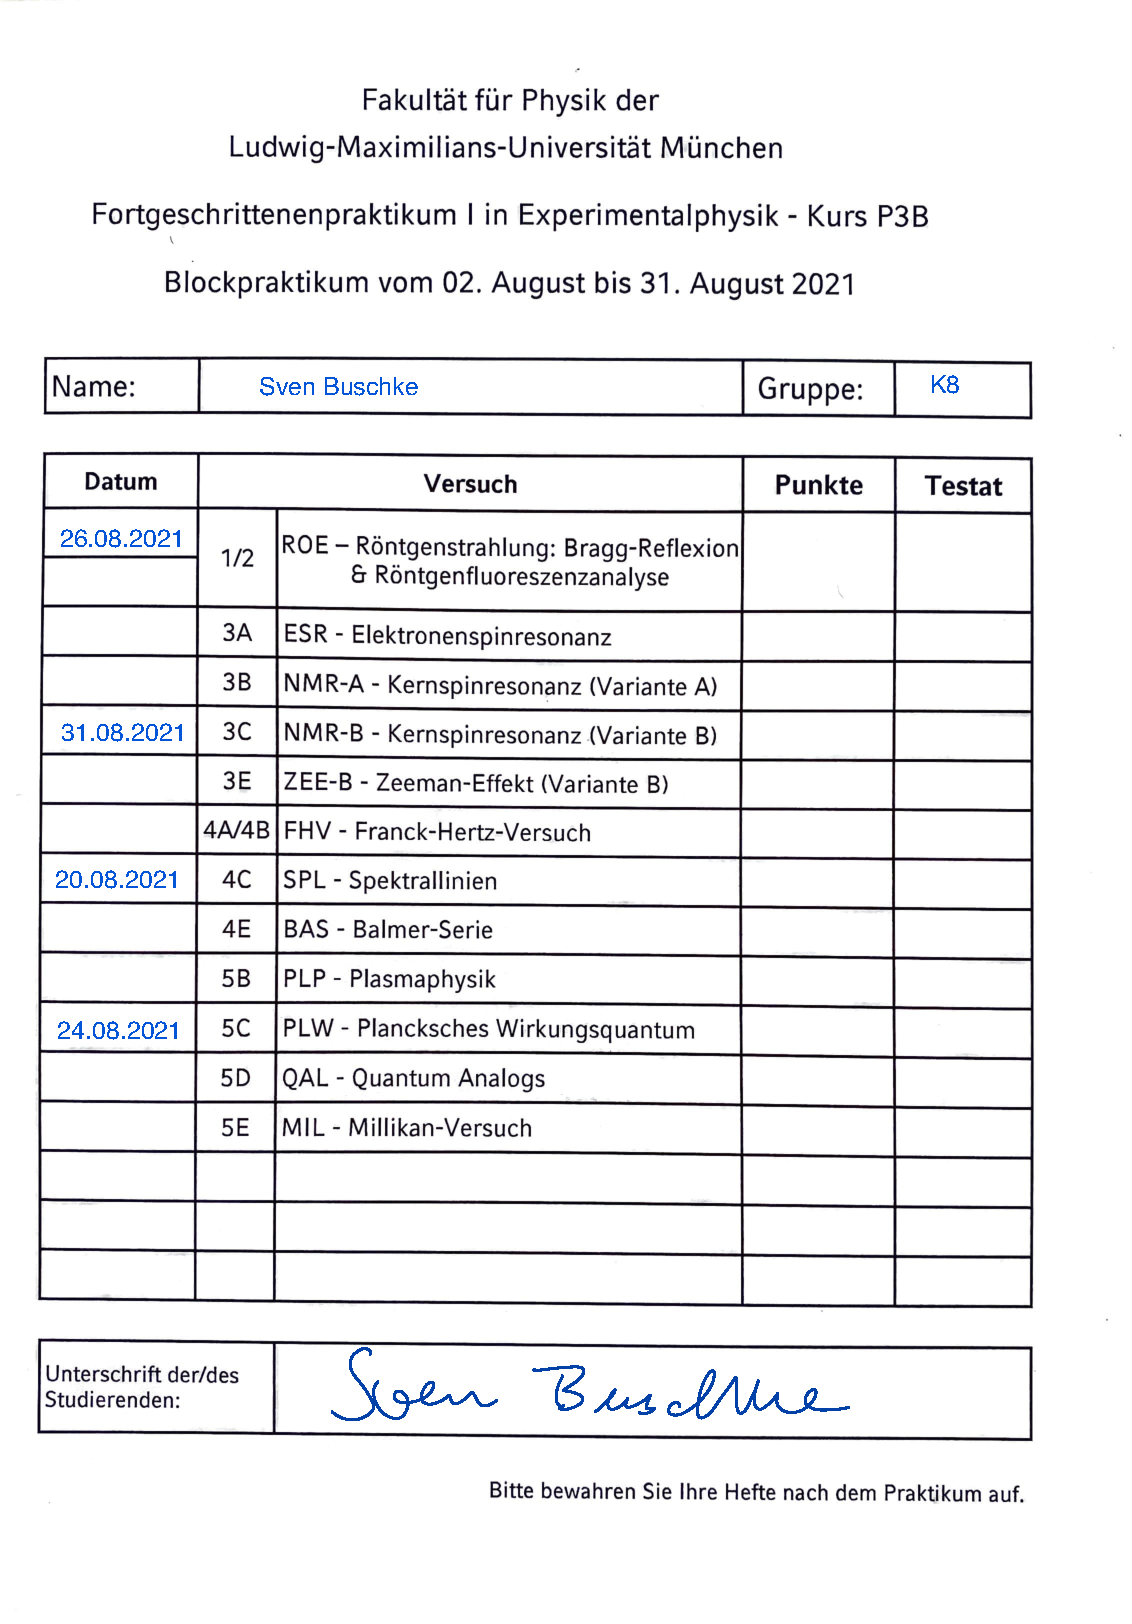
\includepdf[pages=1,scale=0.9,pagecommand={}]{Deckblatt-P3B-signed-20210825.pdf}
       %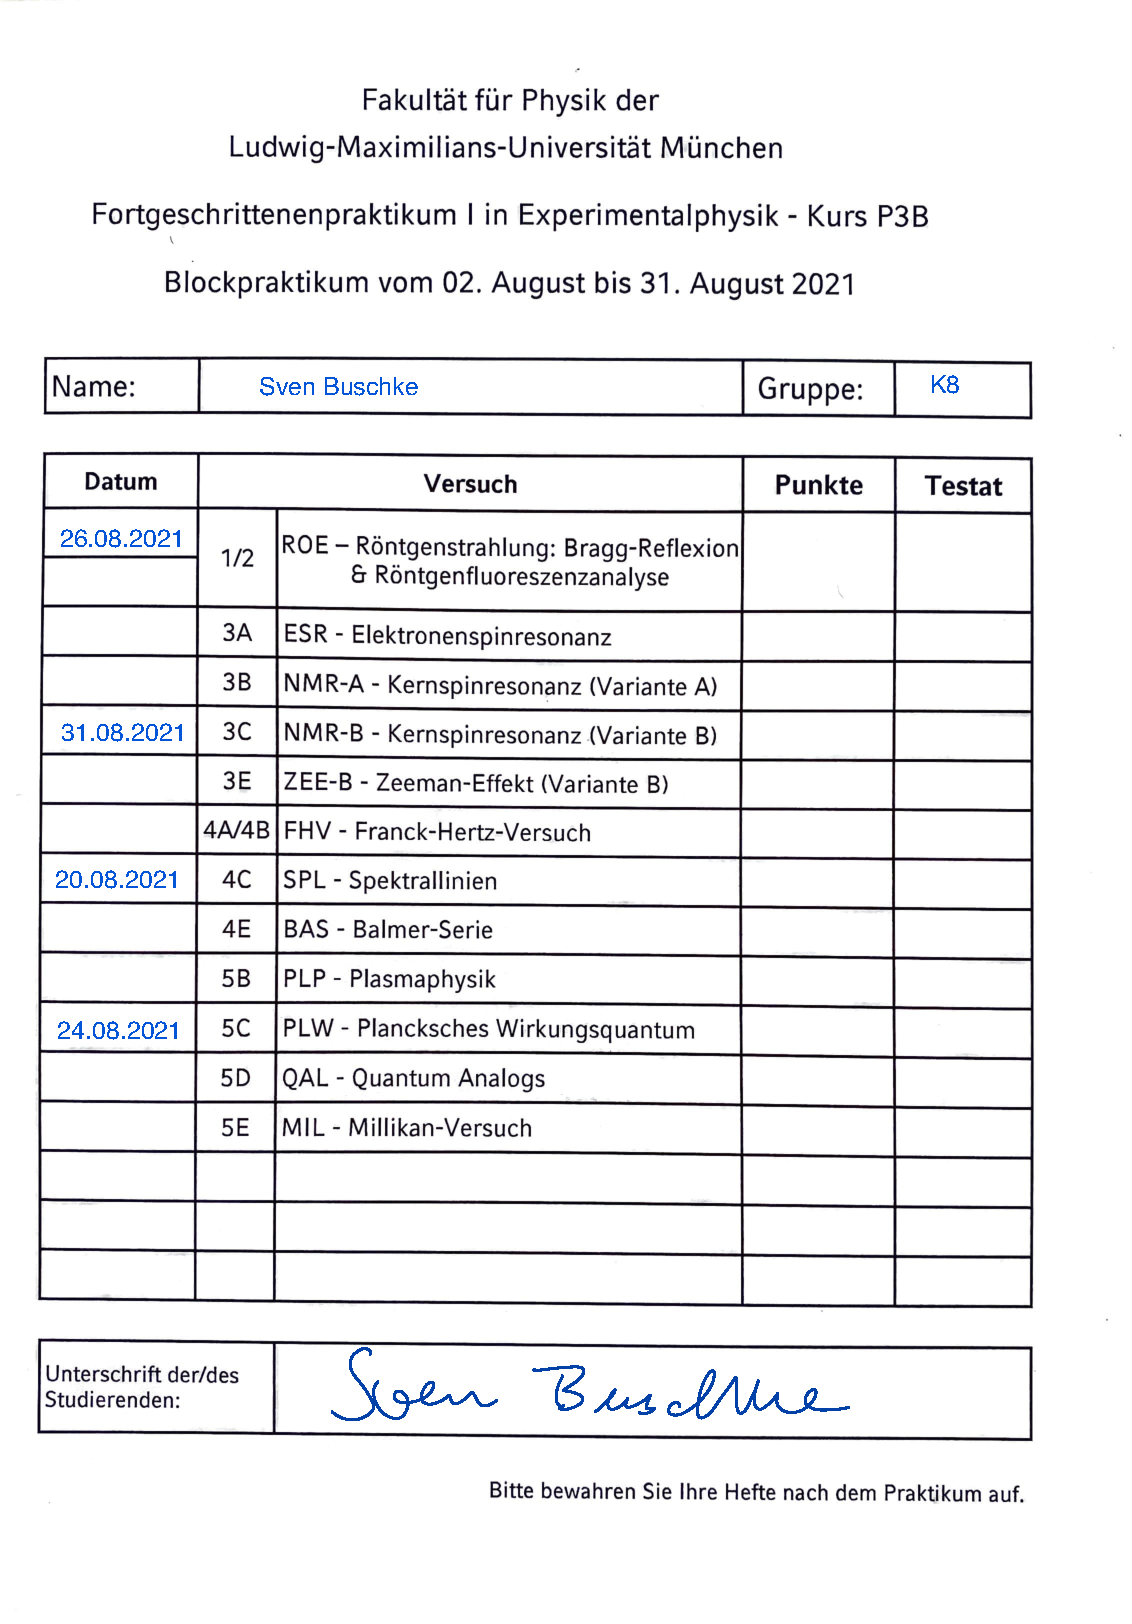
\includegraphics[width=.96\columnwidth]{Deckblatt-P3B-signed-20210825.pdf}
       \newpage
       
\includegraphics[width=0.165\columnwidth]{lmu-seal.pdf}
       
\includegraphics[width=0.35\columnwidth]{lmu-logo.pdf}
       \vskip 0.5cm   
       \textsc{\Large P3B-Praktikum}\\[0.5 cm]
	     {\large \@date\par}
       \vskip 1.0cm
	\rule{\linewidth}{0.2 mm} \\[0.4 cm]
	{ \huge \bfseries \@title}\\
	\rule{\linewidth}{0.2 mm} \\[1.5 cm]
	
	\begin{minipage}{0.5\textwidth}
		\begin{flushleft} \large
			\emph{Name:} \studentfullname\\
			Matrikelnummer: \matrikelnumber
			\end{flushleft}
			\end{minipage}
			\begin{minipage}{0.4\textwidth}
			\begin{flushleft} \large
			Versuchstermin: \dateexperiment\\
			Versuchsdauer: \timeexperiment
		\end{flushleft}
	\end{minipage}\\[2 cm]
   \end{center}
   \vfill
   \null
   \cleardoublepage
  }
\makeatother



%-------------------------------------------------------------------------------------------
%	START OF DOCUMENT
%--------------------------------------------------------------------------------------------

\begin{document}
%\large 
\maketitle
\frontmatter
\let\cleardoublepage\clearpage
\mainmatter
\sloppy



%--------------------------------------------------------------------------------------------
%	RESULTS AND ANALYSIS
%--------------------------------------------------------------------------------------------

\setcounter{tocdepth}{3}
\tableofcontents

\section{Vorbereitung Versuch 3C NMR-B --- Gepulste Kernspinresonanz}
\subsection{Physikalische Grundlagen}

\subsubsection{Stichworte}
\paragraph{Blochkugel}
Die Bloch-Kugel ist eine grafisch-geometrische Darstellung in der Quantenmechanik. Sie stellt die Überlagerungen der Zustände eines Zweizustandssystems als Punkte auf einer Kugeloberfläche dar. Dabei wird der Vektor in eine Kugel eingezeichnet mit den Polarkoordianten $\phi$ und $\theta$. Den Nordpol der Kugel bildet der „up“ Zustand und den Südpol der „down“ Zustand. Die beeiden Eigenzustände liegen sich also gegenüber. Befände sich ein quantenmechanischer Zustand nur in einem der Eigenzustände würde der Blochvektor genau auf der z-Achse der Blochkugel liegen. Außerdem zeigt der Blochvektor in die Magnetisieren des Protons. Falls es eine zeitabhängigkeit gibt, bewegt sich der Vektor mit der entsprechenden Frequenz um die z-Achse der Kugel.\footnote{https://de.wikipedia.org/wiki/Bloch-Kugel}, \footnote{Demtroeder, III, zu präzisieren}

\paragraph{Gyromagnetisches Verhältnis}
Das Analogen zum Gesamtdrehimpuls in der Kernphysik ist der Kernspin. Ersetzt sich aus dem Spin und dem Bahndrehimpuls der Elektronen zusammen. Das gyromagnetische Verhältnis entspricht dem Proportionalitätsfaktor zwischen einem Drehimpuls eines Teilchens und dem dazugehörigen mag.\footnote{https://de.wikipedia.org/wiki/Gyromagnetisches_Verhaeltnis}

\paragraph{Energieniveaus eines Systems mit Spin im Magnetfeld}
Wird ein Kern einem externen Magnetfeld ausgesetzt, spalten sich die einzelnen Energieniveaus gemäß des Zeeman-Effekts auf.

\paragraph{Energieniveaubesetzung (Boltzmann-Ststistik)}
ach der Holzmann-Statistik ist die Wahrscheinlichkeit ein System in einem bestimmten Zustand im thermischen Gleichgewicht zu finden gegeben durch:$p = \frac{1}{Z} e^{-Elk_bT}$ mit $Z = \sum e^{-Elk_bT}.$\footnote{https://de.wikipedia.org/wiki/Boltzmann-Statistik}


\paragraph{Präzession der Magnetisierung}
Ist der Winkel eines Zustands auf der Blochkugel zeitabhängig z.B so präzidiert dieser mit der Frequenz 
um die z-Achse der Kugel. 

\paragraph{$\pi / 2, \pi$-Puls}
Die Stärke eines Pulses ist gegeben durch $A=\omega \tau$, mit der Länge $\tau$ des Pulses. Sie entspricht jeweils $\pi$ bzw. $\pi/2$. Bei einem $\pi$-Puls wird die Magnetisierung umgepolt. An der Blochkugel bedeutet dies, dass er genau in die entgegengesetzte Richtung zeigt. Bei einem $\pi/2$ Puls ändert sich die Magnetisierung gerade um 90 Grad in die entsprechende Richtung.

\paragraph{1-D Bildgebung mittels Fourier-Transformation}
Wenn entlang der y-Achse ein linearer Magnetfeldgradient angelegt wird haben, die die Protonen an verschiedenen stellen entlang der Achse unterschiedliche Lamor-
Frequenzen. Durch Fourier Transformation der empfangenen Singnale lässt sich die räumliche Verteilung der Protonen bestimmen, da die Höhe des Signals direkt Proportional zur Schichtdicke der Protonen ist.

\subsubsection{Theoretischer Hintergrund / Überblick Versuche}
\paragraph{Teilversuch 1 - Vorversuch: Vorarbeiten: Versuchsaufbau kennenlernen, Beobachten eines ersten Signals, Optimierung der Parameter}
\paragraph{Teilversuch 2: Ein-Puls-Betrieb: Bestimmung der Zerfallszeit T2}
\paragraph{Teilversuch 3: Zwei-Puls-Betrieb: Pi-2Pi-Pulsfolge, Spin-Spin-Relaxationszeit T2}
\paragraph{Teilversuch 4: Zwei-Puls-Betrieb: Pi-Pi-Pulsfolge, Spin-Gitter-Relaxationszeit T1}
\paragraph{Teilversuch 5: 1D-Bildgebung mittels Fourier-Transformation}
\paragraph{Teilversuch 6: Materialbestimmung}

\section{Versuchsdurchführung und Auswertung}
\subsection{Teilversuch 1 - Vorversuch: Vorarbeiten: Versuchsaufbau kennenlernen, Beobachten eines ersten Signals, Optimierung der Parameter}
\subsubsection{Versuchsvorbereitung, Grundlagen des Versuches, Erläuterung verwendeter Formelzeichen, Versuchsziel, Erläuterung der Messmethoden, schematische Skizzen, Planung der Durchführung, Versuchsplanung, Versuchsdurchführung}
Ziel dieses Teilversuches ist es die Apparatur Schritt für Schritt einzustellen, um die folgenden Messungen sauber durchführen zu können.

\subsubsection{Versuchsergebnisse und -auswertung}
Versuchsergebnisse und Auswertung.

\subsection{Teilversuch 2: Ein-Puls-Betrieb: Bestimmung der Zerfallszeit T2}
\subsubsection{Versuchsvorbereitung, Grundlagen des Versuches, Erläuterung verwendeter Formelzeichen, Versuchsziel, Erläuterung der Messmethoden, schematische Skizzen, Planung der Durchführung, Versuchsplanung, Versuchsdurchführung}
In diesem Teilversuch sollen Sie die Relaxationszeit des freien Induktionszerfalles bestimmen.

\subsubsection{Versuchsergebnisse und -auswertung}
Versuchsergebnisse und Auswertung.

\subsection{Teilversuch 3: Zwei-Puls-Betrieb: Pi-2Pi-Pulsfolge, Spin-Spin-Relaxationszeit T2}
\subsubsection{Versuchsvorbereitung, Grundlagen des Versuches, Erläuterung verwendeter Formelzeichen, Versuchsziel, Erläuterung der Messmethoden, schematische Skizzen, Planung der Durchführung, Versuchsplanung, Versuchsdurchführung}
Ziel dieses Teilversuches ist die Bestimmung der „echten“ Spin-Spin-Relaxationszeit T2.

\subsubsection{Versuchsergebnisse und -auswertung}
Versuchsergebnisse und Auswertung.

\subsection{Teilversuch 4: Zwei-Puls-Betrieb: Pi-Pi-Pulsfolge, Spin-Gitter-Relaxationszeit T1}
\subsubsection{Versuchsvorbereitung, Grundlagen des Versuches, Erläuterung verwendeter Formelzeichen, Versuchsziel, Erläuterung der Messmethoden, schematische Skizzen, Planung der Durchführung, Versuchsplanung, Versuchsdurchführung}
In diesem Teilversuch sollen Sie die Spin-Gitter-Relaxationszeit T1 bestimmen.

\subsubsection{Versuchsergebnisse und -auswertung}
Versuchsergebnisse und Auswertung.

\subsection{Teilversuch 5: 1D-Bildgebung mittels Fourier-Transformation}
\subsubsection{Versuchsvorbereitung, Grundlagen des Versuches, Erläuterung verwendeter Formelzeichen, Versuchsziel, Erläuterung der Messmethoden, schematische Skizzen, Planung der Durchführung, Versuchsplanung, Versuchsdurchführung}
Ziel dieses Versuches ist die Untersuchung des Spektrums einer unbekannten, undurchsichtigen Probe. 

\subsubsection{Versuchsergebnisse und -auswertung}
Versuchsergebnisse und Auswertung.
https://www.overleaf.com/project/612b9974a652806b244bd989
\subsection{Teilversuch 6: Materialauswertung}
\subsubsection{Versuchsvorbereitung, Grundlagen des Versuches, Erläuterung verwendeter Formelzeichen, Versuchsziel, Erläuterung der Messmethoden, schematische Skizzen, Planung der Durchführung, Versuchsplanung, Versuchsdurchführung}
Hier soll durch die Bestimmung der Longitudinalen Relaxationszeit T1 einer enthaltenen Schicht eine Materialbestimmung durchgeführt werden. 

\subsubsection{Versuchsergebnisse und -auswertung}
Versuchsergebnisse und Auswertung.


\section{Anhang - Laborheft}
%\includepdf[pages=-,scale=0.9,pagecommand={}]{P3B-ROE.pdf}
hier kommt das Laborheft

\end{document}